\documentclass{article}

\usepackage{geometry}
 \geometry{
 a4paper,
 total={170mm,257mm},
 left=20mm,
 top=20mm
 }
\usepackage{float}
\usepackage{graphicx}
\usepackage{indentfirst}
\usepackage{hyperref}

\graphicspath{ {./images/} }
\renewcommand*\contentsname{Daftar Isi}
\renewcommand{\figurename}{Figur}
\renewcommand{\tablename}{Tabel}

\begin{document}
	\begin{titlepage}
		\begin{center}
			
			\null
			{
				\huge \bfseries Tugas Praktikum Pengembangan Perangkat Lunak}\\
			[1cm]
			{\LARGE Business Process KataHati}\\
			
			\vspace{2cm}
			
			\begin{figure}[H]
				\centering
				
\includegraphics[width=200px]{/HitamPutih.jpg}
			\end{figure}
			
			\vspace{3cm}
			
			{\Large 
				Disusun oleh Kelompok YapaYapaHuy} {\Large :\\
				\vspace{0.5cm}
				Ardacandra Subiantoro (18/427572/PA/18532)\\
				Chrystian (18/430257/PA/18770)\\
				Juandito Batara Kuncoro (18/427582/PA/18542)\\
			}
			
			
			\vspace{2cm}
			
			{\normalsize \bfseries
				PROGRAM STUDI S1 ILMU KOMPUTER\\
				DEPARTEMEN ILMU KOMPUTER DAN ELEKTRONIKA\\
				FAKULTAS MATEMATIKA DAN ILMU PENGETAHUAN ALAM\\
				UNIVERSITAS GADJAH MADA\\
				YOGYAKARTA\\
				\vspace{0.2cm}
				2020
			}
			
		\end{center}
	\end{titlepage}

	\newpage
	\pagenumbering{arabic}
	
	\section{Deskripsi Permasalahan}
	\par
	Keadaan pandemi COVID-19 menyebabkan banyak mahasiswa kekurangan interaksi sosial sehingga mereka tidak dapat memenuhi kebutuhan sosial mereka. Hal ini dapat menyebabkan stres berlebih dan kurangnya produktivitas. Tujuan program ini adalah membantu mahasiswa yang mengalami masalah mental oleh karena keadaan pandemi dengan memberikan mereka saran dan bantuan profesional.
	\par
	Untuk memenuhi kebutuhan tersebut desain perangkat lunak harus memiliki tingkat aksesibilitas yang tinggi untuk dapat diraih dan diketahui oleh mahasiswa yang bermasalah tersebut. Dengan profesional ahli, sistem harus dapat mengatur pertemuan, melakukan penjadwalan, serta menghubungkan profesional dengan mahasiswa bermasalah secara cepat, tepat, dan efisien.
	
	\section{Bisnis Proses}
	\begin{figure}[H]
	\centering	
	
\includegraphics[width=150px]{/logo/logo_katahati.png}
	\caption{Logo KataHati}
	\end{figure}
	\par
	Bisnis proses pada perangkat lunak KataHati melibatkan beberapa pihak : mahasiswa, tenaga profesional, dan admin.
	\par
	Mahasiswa pertama-tama membuat akun dengan mendaftarkan email mereka dan melakukan proses verifikasi. Lalu, mereka mengisi form yang berisi pertanyaan-pertanyaan mengenai gejala-gejala yang biasanya tampak pada orang-orang dengan masalah mental. Hasil dari form tersebut akan mengklasifikasikan masalah mental yang dialami mahasiswa (depresi, bipolar, OCD, dll) dan digunakan untuk mengarahkan mahasiswa tersebut kepada tenaga profesional dengan spesialisasi yang sesuai. Mahasiswa lalu memilih slot jadwal yang tersedia dari tenaga profesional yang ada dan membuat janji temu secara daring. Pada waktu yang sudah dipilih, mahasiswa akan bertemu dengan tenaga profesional melalui media chat untuk mendapatkan saran akan masalah mereka. Mahasiswa dapat memilih untuk konsultasi secara anonim bila mereka tidak ingin memberikan identitas mereka. Mahasiswa juga dapat bergabung dengan sharing group berisi mahasiswa-mahasiswa lain dengan masalah yang mirip untuk saling mendukung satu sama lain.
	\par
	Tenaga profesional adalah dokter, tenaga magang, psikolog, atau mahasiswa dengan keahlian di bidang kesehatan mental yang bersedia membantu mahasiswa-mahasiswa yang memiliki masalah mental. Tenaga profesional memberikan jadwal dimana mereka memiliki waktu kosong dan dapat memberikan konsultasi daring. Lalu, tenaga profesional bertemu secara daring melalui chat dengan mahasiswa-mahasiswa yang sudah membuat janji untuk memberikan bantuan dan saran.
	\par
	Admin adalah karyawan yang fasih komputer dan memiliki tugas memastikan semua proses dalam perangkat lunak ini berjalan dengan lancar. Tugas mereka antara lain adalah memastikan sistem penjadwalan berjalan dengan sesuai, memoderasikan sharing group agar tidak menyimpang dari tujuan awalnya, berinteraksi dengan mahasiswa dan tenaga profesional yang memiliki masalah teknis, dan mengurus database. 
	
	\section{Proses Design}
	\begin{enumerate}
		\item Proses Pendaftaran \\
		Mahasiswa mendaftar dan melakukan proses verifikasi.
		\item Proses Pengisian Form \\
		Mahasiswa mengisi form untuk  klasifikasi masalah yang mereka alami, lalu mereka diarahkan kepada profesional yang sesuai.
		\item Proses Penjadwalan \\
		Mahasiswa memilih jadwal untuk berinteraksi dengan tenaga profesional sesuai waktu yang tersedia.
		\item Proses Interaksi \\
		Mahasiswa interaksi dengan profesional dengan media seperti chat.
		\item Proses Sharing Group \\
		Mahasiswa dapat bergabung ke dalam chat room berisi mahasiswa-mahasiswa lain yang memiliki masalah serupa.
	\end{enumerate}
	
	\begin{figure}[H]
		\centering	
		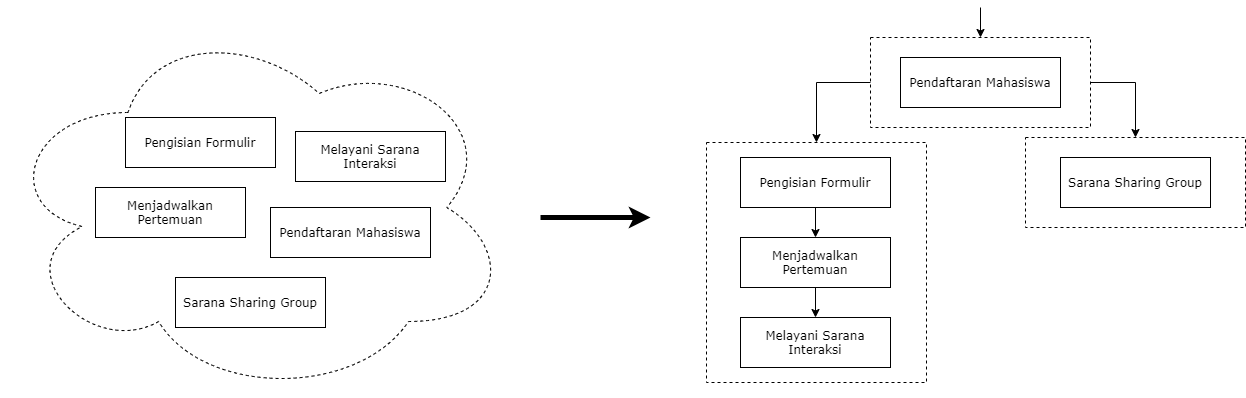
\includegraphics[width=500px]{/diagram/diagram_processes.png}
		\caption{Diagram Pembagian Subscope pada Sistem}
	\end{figure}
	\section{Spesifikasi User}
	\begin{enumerate}
		\item Admin \\
		Karyawan yang dapat mengkonfigurasikan sistem, termasuk proses penjadwalan, manajemen database, menjadi moderator chat room. Admin merupakan pengguna spesial dan memiliki otoritas dengan tingkat paling tinggi untuk mengakses seluruh bagian dari perangkat lunak.
		\item Mahasiswa \\
		Pengguna website yang fasih dengan komputer dan sedang membutuhkan bantuan secara mental.
		\item Profesional \\
		Tenaga profesional di bidang kesehatan mental yang dapat memberikan bantuan berupa saran-saran kepada mahasiswa yang mengalami masalah mental.
	\end{enumerate}
	
\end{document}